The Standard Model of particle physics is one of the most precisely tested
theories. It is a relatistivic quantum field theory using the Lagrange
formalism.

It provides a unified description of three of the four forces of nature: the
electromagnetic interaction, the weak interaction, and the strong
interaction. Gravitation not included.

Natural units $\hbar = c = 1$. Can be recovered by dimensional
analysis. Heaviside--Lorentz units?

Einstein summation convention: Sum over repeated indices.

Cross-sections in barn $\SI{1}{\barn} = 10^{-28}\,\si{\metre\squared}$

Cite what this description is based on: \cite{Thomson:2013zua}


\section{Particles and Interactions in the Standard Model}

The Standard Model, shown in~\Cref{fig:sm_particles}, consists of 12 elementary
spin-$\frac{1}{2}$ particles referred to as \emph{fermions} and their
anti-particles, and five types of particles with integer spin referred to as
\emph{bosons}. With the discovery of the Higgs boson in
2012~\cite{HIGG-2012-27,CMS-HIG-12-028}, experimental evidence for the existence
of all fermions and bosons predicted by the Standard Model is established.

\begin{figure}[htbp]
  \centering

  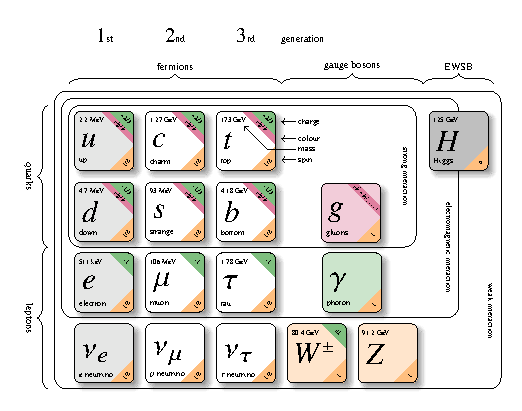
\includegraphics[width=\textwidth]{theory/sm}

  \caption{Particles of the SM. The diagram is adapted from Ref.~\Cref{sm_tikz}
    with updated particle properties from Ref.~X. Antiparticles are not shown
    explicitly have additive quantum numbers of opposite sign but otherwise the
    same properties of the respective particle.}
  \label{fig:sm_particles}
\end{figure}


The elementary particles of the SM can be divided into three categories:
\begin{description}

\item[Fermions] predicted by the SM have spin-$\frac{1}{2}$. Consequently, they
  are massive\footnote{Neutrinos are considered as massless in the SM, however,
    the observation of neutrino
    oscillations~\cite{Super-Kamiokande:1998kpq,SNO:2002tuh} is experimental
    evidence for neutrinos having small but non-zero mass.} and adhere to the
  Pauli exclusion principle and are therefore considered to be \emph{matter}
  particles. The fermions of the SM are divided into \emph{quarks} that take
  part in the strong interaction, and \emph{leptons} that do not.

  Divided into six \emph{flavours}???

  Up-type ($u$, $c$, $t$) and down-type ($d$, $s$, $b$) quarks.

  All fermions take part in the weak interactions while only quarks and
  electrically charged leptons ($e$, $\mu$, $\tau$) take part in the
  electromagnetic interaction. For every fermion, a corresponding anti-particle
  exists that has the same properties but with opposite additive quantum
  numbers.


  % All ordinary (stable) matter consists of fermions of the first generation,
  % i.e.\ up- and down-quarks as well as electrons. The only difference between
  % fermions of different generations is their mass.

  Quantum numbers: colour charge, electric charge, weak isospin (weak hypercharge)

\item[Gauge bosons] predicted by the SM are particles with spin-$1$ and are
  therefore also referred to as vector bosons. The gauge bosons mediate the
  three of the fundamental forces of nature. The strong interaction is mediate
  by the exchange of massless gluons that couple to colour charge carried by
  quarks and gluons. The massless photon couples to electric charge and thereby
  mediates the electromagnetic interaction. Finally, the massive $W^\pm$ and $Z$
  boson

\item[The Higgs boson]

\end{description}


Four types of vector (spin-1) bosons in.

The vector bosons mediate the fundamental interactions.

(Eight) gluons mediate the strong interaction.

The photon mediates the electromagnetic interaction.

The massive vector bosons $W^\pm$ and $Z$ mediate the weak interaction.

The mediators arise from theories adhering to certaing symmetry principles,
referred to as gauge theories, are therefore also referred to as \emph{gauge
  bosons}. A more detailed description of the interactions follows...

A special role in the SM is taken by the Higgs boson, the only scalar (spin-0)
boson in the SM. The Higgs boson is necessary to allow the $W^\pm$ and $Z$
bosons to be massive without violating the underlying symmetry principles of the
SM.

Bosons:

One scalar Boson, the Higgs boson. Explaining the mass of the heavy gauge bosons
without violating the symmetry assumptions underlying the Standard Model (more
on this later) using the BEH-mechanism.


Daily matter: electrons, up- and down-quarks.


In the SM the neutrinos are assumed to be mass-less which is experimentally
proven to not be the case.


\section{Symmetries and Interactions}

Guiding principle of the SM: local gauge invariance.


\subsection{The Langrange Formalism}

The description of the Standard Model uses the Lagrange formalism describing the
behaviour of fields, $\phi_i(\myvec{x})$, with a \emph{Lagrangian density}
$\lagrange(\phi_i, \partial_\mu \phi_i)$, where $\partial_\mu$ is the derivative
with respect to the $\mu$-th space-time coordinate. Hereafter, the Lagragian
density is referred to as the Lagrangian.

The ``equations of motion'' for the fields are obtained by the principle of
least action yielding Euler--Lagrange equations:
\begin{align*}
  \partial_{\mu} \left( \frac{\partial \lagrange}{\partial (\partial_{\mu} \phi_i)} \right) - \frac{\partial \lagrange}{\partial \phi_i} = 0
\end{align*}

$\partial_{\mu}$ is the covariant derivative $\partial / \partial x^{\mu}$.




\subsection{Local Gauge Invariance}

Interactions are dictated by symmetry principles


Symmetry group of the SM:
\begin{align*}
  SU(3)_{\text{color}} \times SU(2)_{\text{L}} \times U(1)_{Y}
\end{align*}

Lie group:
\begin{align*}
  U(\myvec{\alpha}) = \exp(i \myvec{\alpha} \cdot \myvec{G})
\end{align*}
U unitary. G generator (hermitian).


Local gauge invariance:
$\psi(\myvec{x}) \to \psi^\prime(\myvec{x}) = U(\myvec{x}) \psi(\myvec{x})$


\subsection{QED}

\begin{align*}
  \lagrange_{\text{Dirac}} = i \bar{\psi} \gamma^{\mu} \partial_{\mu} \psi - m \bar{\psi} \psi \quad \to \quad (i \gamma^{\mu} \partial_{\mu} - m) \psi = 0
\end{align*}

Dirac equation describing free fermions.

Perform local U(1) phase transformation.

The Dirac equation of a free fermion does not satisfy local gauge invariance due
to derivative terms.

Can introduce an alternative derivative: $D_\mu = \partial_\mu + i q A_\mu$.

Dirac spinor: $\psi$.


\subsection{QCD}

\subsection{Weak}

charged-current interaction $SU(2)$ symmetry -> weak isospin

Left handed chiral particles are in a weak isospin doublet

Right handed chiral particles are in a weak isospin singlett

Vice versa for antiparticles


\subsection{Electroweak Unification}

\section{Electroweak Symmetry Breaking}

\section{Fermion Masses}

\section{The Higgs Boson}


\clearpage

%%% Local Variables:
%%% mode: latex
%%% TeX-master: "../../phd_thesis"
%%% End:
